
\documentclass[11pt]{article}
\title{Unicef User Testing Task Form}
\author{Matteo Sissa, Lorenzo Prosch, Annachiara, Ivan Della Vecchia}

\usepackage{hyperref}
\usepackage{geometry}
\usepackage[]{eforms}
\usepackage{graphicx}
\usepackage[table]{xcolor}	

\geometry{
	top=2cm,
	right=2cm,
	left=2cm,
	bottom=2cm
}
\definecolor{linkblue}{RGB}{0, 0, 255}
\hypersetup{
	colorlinks=true,
	linkcolor=linkblue,
	urlcolor=linkblue
}



\begin{document}
	\maketitle
	\renewcommand{\arraystretch}{3.5}
	
	\vspace{0.5cm}
	
	\begin{Form}
		
		\begin{tabular}{p{10cm} p{10cm}}
	
	\TextField[width=4cm, bordercolor=]{Name: } &
	\TextField[width=4cm, bordercolor=]{Surname: }\\
	\ChoiceMenu[combo, name=countryField, bordercolor=, width=5cm]{Age: }{20, 21, 22, 23, 24, 25, 26, 27, 28, 29, 30} &
	\TextField[width=3cm, bordercolor=, format={dd/mm/yyyy}]{Date: }\\
	
	\end{tabular}
	
	\vspace{1cm}
	
	\subsection*{Introduction}
	
	
	User testing is a common usability testing practice that is applied to evaluate the interaction between a product and its target users. 
	It is a very precious source of information for developers and designers as it provides a direct access to the perception of the product from the end users.\\
	In this specific case, user testing is applied to the \href{https://www.unicef.org/}{official Unicef website} and it aims to verify some aspects of its usability. To achieve this, some tasks will be illustrated in the following of this document and the user is asked to complete them. 
	It is important to remark that this is not a test on the user, rather on the website, whose flaws have to emerge thanks to the user collaboration. \\
	As a final note, all data gathered through these forms will be anonymised before being displayed in any public document or presentation.
	
	\vspace{1cm}
	
	\subsection*{Task List}
	In the following, there are six tasks that the user is asked to complete on the \href{https://www.unicef.org/}{official Unicef website}.
	\begin{enumerate}
		
		\item Unicef is invested in many humanitarian problems and among them there are relevant hot topics like gender equality, nutrition (especially children nutrition), climate change, COVID-19 response... For every important area of interest for Unicef, the website first offers a high-level page with an \textbf{overview} of the work Unicef is doing in that regard. Then, inside these high-level pages, the user can find \textbf{resources} (reports, articles...) that further deepen the general subject.\clearpage
	
		As an example, Unicef's website offers a page dedicated to the matter of children with disabilities and inside this high-level page it is possible to spot resources related to the topic that are displayed with the following graphics:
		\begin{center}
			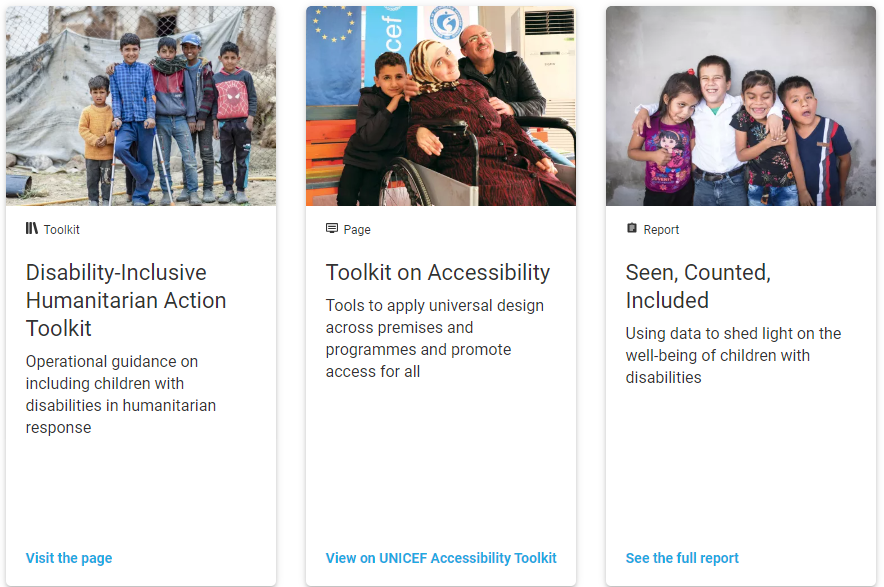
\includegraphics[width=0.3\linewidth]{res/Resources}
		\end{center}
		
		The first task is about getting familiar with these presentation pages present on the website. So, suppose you were interested in the theme of \textbf{gender equality}, can you spot the web page providing an overview of the work Unicef is doing in that area? Once there, are you able to list \textbf{ALL} the \textbf{resources} related to gender equality?
		Now, try to repeat the same procedure also for the topics of \textbf{COVID-19 response} and \textbf{nutrition}.
		
		\item Unicef achieves many of its goals also thanks to the generous \textbf{donations} of people from all around the world who believe in the organization's principles and ideas. Consequently, one of the most relevant actions that a user can take on the official Unicef website is the one of donating for one of the causes presented on the web page. To test this feature, suppose to be willing to donate \textbf{specifically} for the \textbf{Afghanistan emergency} (so \textit{NOT} a general donation to Unicef), can you find the correct area of the website to carry out this task?
		
		\item Unicef operates in many different countries of the world with different purposes and goals. As a consequence of this, the website is structured in such a way that there are subpages dedicated to each specific country in which Unicef works. Suppose you were interested in reading specifically what Unicef is doing or organising in Italy, can you find the webpage of \textbf{Unicef Italy} navigating from the main one?
		
		\item \textit{The State of the World's Children} is an annual report that Unicef publishes to illustrate the most relevant threats in today's world to children survival. It is the flagship of the organisation, so it is extremely important. Suppose you wanted to find this report \textbf{for the year 2023}, in which the problem of \textbf{children vaccination} is explained and illustrated. Are you able to spot it and discover the \textbf{four solutions} that Unicef proposes to vaccinate as many children as possible against the most life-threatening diseases and illnesses?\\
		N.B. The report shouldn't be downloaded, the overview page is enough to answer.
		
		\item Apart from donating money, an alternative way to contribute to Unicef's causes is to \textbf{collaborate as an intern} in one of the partner companies or in Unicef itself. The website should be able to attract interns from all over the world and make the process of \textbf{applying for jobs} as straightforward as possible. Now let's assume you were navigating on this website to find job opportunities for an internship, can you identify the right section of the website to look into and list all the \textbf{internship} opportunities that are offered in \textbf{South Africa} specifically?
		
		\item For every major topic on Uncef's website, there are many related articles and resources that are offered and the user is able to browse them and read what s/he's interested into. This task is about finding a \textit{specific} article on the website, without knowing its exact location in advance. So, let's assume you were interested in reading an article on the\textbf{ COVID-19 vaccination situation in Bangladesh}. The article's title is specifically \textit{Bangladesh's COVID-19 vaccination rate has soared in a year}. Are you able to intuitively navigate from the home page of the Unicef website to the right location where this article might be placed?
		
		
	\end{enumerate}
			

	
	\end{Form}
	
	\clearpage
	
	
	\subsection*{Notes for the inspector}
	Here are some relevant notes regarding the solutions to the tasks and the most straightforward and expectable navigation paths that the users are likely to use to accomplish the tasks. These paths have been elicited from an accurate inspection of the \href{https://www.unicef.org/}{Unicef website} and they can be considered as the most direct ways to achieve the goals requested by the tasks.
	\begin{enumerate}
		\item The first task is about highlighting the inconsistencies of the pages under "All areas" section (which are very relevant since they are the first sections of the website that a new user sees). 
		More specifically, the task is designed to make the user notice the differences in the ways related resources are provided on the website for the different topics. The selected subjects are:
		\begin{itemize}
			\item \href{https://www.unicef.org/gender-equality}{Gender Equality}: all resources can be listed by scrolling the gender equality page and finding the correct section for resources at the end of the page (there is a button there).
			\item \href{https://www.unicef.org/coronavirus/covid-19}{COVID-19 response}: this page shows a totally different way of offering resources, with a list of articles, publications that can be lengthened by clicking on a button.
			\item \href{https://www.unicef.org/nutrition}{Nutrition}: in this case, the resources are organised in a table with links placed at the end of the page.
		\end{itemize}
		\item The second task aims to show the different behaviours of the DONATE buttons spread across the different pages of \href{https://www.unicef.org/}{Unicef website}. From the home page of the website, the button leads to a general donation to Unicef. In some subpages of the website the same button leads to a donation for supporting the specific cause described in that subpage. To donate specifically for the Afghanistan crisis and solve the task, the user has to go under Stories - \href{https://www.unicef.org/emergencies/delivering-support-afghanistans-children}{Afghanistan} and then click on the DONATE button from there.
		\item The user is expected to navigate on this path: About Unicef - All locations and then use the menu there to select the \href{https://www.unicef.it/}{Unicef Italy} website.
		\item The most straightforward path is under the section Research and Reports - \textit{The State of the World's Children}. It is important to notice here that the solutions provided by Unicef are the ones under "The Solutions" section, more specifically the subtitles under that section, so:
		\begin{itemize}
			\item Vaccinate every child through effective immunization programmes and catch-up campaigns.
			\item Strengthen confidence in vaccination.
			\item Invest in immunization and health.  
			\item Build resilient health systems. 
		\end{itemize}
		The fact that these subsections are divided with images and alternated with other not-related elements creates confusion in the user, and that's what has to be elicited from this task.
		\item The path to be followed is: Take Action - Work with us - Search Jobs (button) then use filters for the internship and the country (South Africa).
		\item The article can be found under the \href{https://www.unicef.org/coronavirus/covid-19}{COVID-19 response} section, at the end of the page where the articles are placed.
	\end{enumerate}
	
	
	
\end{document}